\documentclass[english,letterpaper,12pt,final]{article}
\usepackage{graphicx}
\usepackage{etex}

\sloppy
%\special{papersize=8.5in,11in}% This command prevents the use of other paper size in the dvi2ps conversion
%------Document properties------------
\usepackage{setspace}
\usepackage{pdfpages}
\usepackage{pgfgantt}
\usepackage{enumitem}
%------math packages-------------------
\usepackage{amsthm}
\usepackage{tkz-berge} % Drawing graphs
%------algorithms packages-------------------
%\usepackage[ruled,vlined]{basic/algorithm2e}
\usepackage[noline,linesnumbered,noend]{algorithm2e}
%\linesnumbered
%------bibliography packages-----------
\usepackage{natbib}

\usepackage[utf8]{inputenc}

\usepackage[font=small,labelfont=bf]{caption}
\usepackage{listings}
\usepackage{breakcites}
\usepackage{dsfont}
\usepackage{hyperref}
\usepackage{amssymb,amsthm,amsmath,latexsym}

\usepackage{natbib}

\newcommand{\indep}{\rotatebox[origin=c]{90}{$\models$}}
\newcommand{\leci}{<\!\!\!\!\!\!\!\bigcirc}
%\newcommand{\lessint}{$\bigcirc$}
%------corporative identity of INAOE---
\usepackage{eso-pic}
\usepackage{pstricks}
\usepackage{INAOEMacros}

\usepackage{dsfont}
\usepackage{lineno,hyperref}


\usepackage{amssymb}
\usepackage{pifont}
\usepackage{url}
\usepackage{array}
%\usepackage{subfigure}
\usepackage{lscape}
\usepackage{amsfonts}
\usepackage{amsmath}

\usepackage[normalem]{ulem}
\usepackage{color}
\usepackage{multirow}
%\usepackage{mathtools}

%\usepackage[dvipdfmx]{graphicx} 
%\usepackage{bmpsize}

\usepackage{caption}
\usepackage{subcaption}
%------floating -----------------------
\usepackage{float}
\floatstyle{plain}
\newfloat{codigo}{thp}{lop}[section]
\floatname{codigo}{Algorithm}
\usepackage{booktabs}
%
%usepackage{lscape}
%\usepackage{pdflscape}
%\usepackage{rotating}
\usepackage{tablefootnote}
%------figure packages--------------
%\usepackage{subfigure}

%------page layout---------------------
\oddsidemargin 0.36cm
\evensidemargin 0.36cm
\marginparwidth 0.0cm
\textwidth 16.80cm

\topmargin -1.5cm
\headheight 1.0cm
\headsep 1.0cm
\footskip 1.0cm
\textheight 22.34cm


%\theoremstyle{plain}
%\newtheorem{teo}{Theorem}
%\newtheorem{prop}[teo]{Proposition}
%\newtheorem{defi}[teo]{Definition}
%\newtheorem{obs}[teo]{Observation}
%\newtheorem{lem}[teo]{Lemma}
%\newtheorem{cor}[teo]{Corolary}


%\newcommand{\cmark}{\ding{51}}%
\newcommand{\xmark}{\ding{56}}%
\theoremstyle{definition}
\newtheorem{rmk}{Definition}[section]
\newtheorem{teo}{Theorem}[section]
\newtheorem{thm}{Theorem}[section]
\newtheorem{prop}{Proposition}[section]
\newtheorem{corollary}{Corollary}[section]
\newtheorem{cor}{Corollary}[section]
\newtheorem{problem}{Problem}
\newtheorem{defi}{Definition}[section]
\newtheorem{pf}{Proof}
\newtheorem{pot}{Proof of Theorem \ref{thm2}}



%----------myDeclarations------------
\DeclareMathOperator*{\argmin}{argmin}
\definecolor{blue1}{rgb}{0.58,0.70,0.84}
\definecolor{blue2}{rgb}{0.93,0.95,1.0}
\usepackage{xcolor,colortbl}
\usepackage{titlesec}
\setcounter{secnumdepth}{4}
\titleformat{\paragraph}
{\normalfont\normalsize\bfseries}{\theparagraph}{1em}{}
\titlespacing*{\paragraph}
{0pt}{3.25ex plus 1ex minus .2ex}{1.5ex plus .2ex}

%-----end of preamble------------------
\pagenumbering{roman}
\begin{document}


% Title page
\input{gfrontpage}
%\doublespacing
\singlespacing
\tableofcontents
\newpage
\begin{abstract}
We consider decision problems under uncertainty where the options available to a decision maker and the resulting outcome are related through a causal mechanism which is unknown to the decision maker, although he is aware of the causal nature of his environment. We study how a decision maker can learn about this causal mechanism through sequential decision making as well as using current causal knowledge inside each round in order to make better choices had he not considered causal knowledge. We propose a decision making procedure in which an agent holds \textit{beliefs} about her environment which are used to make a choice and then are updated using the observed outcome. As proof of concept, we present an implementation of this causal decision making model and apply it to a simple problem. We show that the model achieves a performance similar to the classic Q-learning while it also acquires a causal model of the environment. 
\end{abstract}
\pagenumbering{arabic}
\section{Introduction}
\indent A fundamental part of intelligent reasoning is being able to make decisions under uncertain conditions (\cite{danks2014unifying}, \cite{lake2017building}, \cite{pearlwhy}). Uncertain conditions mean that if a set of choices is made available to a decision maker he can not predict the precise consequence of his decision. For this reason, the decision maker must take into account the stochastic relation between actions\footnote{Actions, options and choices to be used equivalently.} and consequences. From the von Neumann-Morgenstern decision making theory we know that if a rational\footnote{To be explained in full detail later.} decision maker knows this stochastic relation, then he \textit{must} choose the action that maximizes the \textit{expected utility} of a \textit{utility function} whose existence is guaranteed (\cite{von1944theory}). On the other hand, if a rational decision maker does not know the probabilities of the ocurrence of certain outcomes, or consequences, given his actions, then he must encode his personal subjective quantifications of any uncertainties in a probability distribution $p$ and choose the action that maximizes expected utility with respect to this probability distribution(\cite{savage1954the}, \cite{bernardo2000bayesian}, \cite{gilboa2009decision}). If the current \textit{knowledge} of a decision maker is not enough to make good choices, then the decision maker can \textit{learn} from the environment by interacting with it in order to update his quantifications of uncertainty (\cite{bernardo2000bayesian}, \cite{peterson2017introduction}).

%In some cases, a decision maker who faces an uncertain environment has enough information to make choices by maximizing expected utility, which is the classic formal criteria for making decisions if rational preferences are assumed (\cite{bernardo2000bayesian}, \cite{gilboa2009decision}). On the other hand, if enough information is not available, the decision maker could attempt to \textit{learn} from the environment by interacting with it.

Learning to perform tasks by interaction has been extensively studied in Computer Science using Reinforcement Learning (RL) (\cite{sutton1998reinforcement}), but the most common used techniques in this field are based on purely associative relations and do not consider any high-level structure of the environment beyond what is expressable in a Markov Decision Process (\cite{garnelo2016towards}). A particular case of a \textit{higher level structure}; i.e., beyond associative patterns, is the case of \textit{causal} structure. A causal structure encondes a series of \textit{cause-effect} relations between events and knowing such relations allows a decision maker to add extra knowledge into the uncertainty of his environment and also allows to plan ahead his actions since he can predict what a certain action will cause (\cite{spirtes2000causation}, \cite{pearl2018theoretical}).\\
\\
Causal reasoning is found at the very core of human reasoning (\cite{danks2014unifying}, \cite{lake2017building}), since it allows us to manipulate our environment and being able to predict effects of a given action (\cite{spirtes2000causation}). It is even argued that in a more basic level the brain is a causal inference machine which uses \textit{effects} to figure out \textit{causes} (\cite{friston2010free}, \cite{hohwy2013predictive}, \cite{clark2015surfing}). Causal claims also support reasoning of the form \textit{if...hadn't occurred then...wouldn't have happened}. It is argued by \cite{pearl2018why} that imagining alternative scenarios is fundamental for humans to make causal reasoning.  Since human beings are known to learn causal models in sequential decision making processes (\cite{sloman2006causal}, \cite{nichols2007decision}, \cite{meder2010observing}, \cite{hagmayer2013repeated}, \cite{danks2014unifying}), and even though this learning is not perfect (\cite{rottman2014reasoning}), our hypothesis is that an autonomous agent can learn and use causal information while interacting with an uncertain environment which is governed by a fixed \textit{causal mechanism} which is unknown to the agent. 

The proposed way for an agent to learn from repeated interactions is by giving him \textit{beliefs} about the structure of the environment, which are to be used as a \textit{true} causal model, and then are to be updated them after an outcome has been observed. While the standard setting in RL is to model the agent-environment interaction as an agent that moves from one \textit{state} to another inside a model of the environment and observing a reward as these transitions occur, we propose to model it as a \textit{game} between the decision maker and a player called \textit{Nature} which will select his actions from the causal model in response to what the decision maker has chosen. The agent, besides learning a policy to choose actions, will also learn a causal model from the environment since the causal model she forms will approximate the true model.

%The agent, using her current beliefs, will generate a \textit{local} causal model and choose an action from it as if that model was the true one. Then, after she observes the consequences of her actions, her beliefs will be updated according to the observed information in order to make a better choice the next time. The agent, besides learning a policy to choose actions will also learn a causal model from the environment since the causal model she forms will approximate the true model.

Learning a causal model of the environment allows to extract high-level insights of a phenomena beyond associative descriptions of what is observed. A causal model is able to \textit{explain} why a particular decision was made since it allows to extract the causes and effects of an agent's actions. Once a causal model is acquired, an external user is able to reason about \textit{what...if...} statements that associative methods can not answer. When a decision maker chooses an action out of many, a causal model allows to ask what would've happened if another action was taken without actually performing the alternative action. It is important to be careful when using the word \textit{explanation} since it allows for several uses in language, here we understand \textit{explanation} as used by \cite{woodward2005making} who considers explanations where what is explained depends on other factors via some relationship that holds as a matter of empirical fact rather than \textit{logical} reasons. Also, learning a causal model of a certain environment would allow transferability of knowledge into similar domains because the underlying cause-effect structure has been captured and could later be used.
\subsection{Outline}
In the Section \ref{Main_Concepts} the main concepts that serve as a foundation for this work will be described; in particular, we will describe in detail what causality means. Since this research proposal asumes that a causal model governs an environment, a precise definition of causality will be given along with the mathematical machinery to perform causal inference. Also, since the entity that will be facing causal environments is a \textit{rational} decision maker we will precisely define, axiomatically, what does rationality means and which are the main theories of rational decision making. At the end of the section, we will describe a mathematical theory which is suitable to modelling interaction between rational decision makers since interactive learning is considered.

After the main concepts have been exposed, in Section \ref{Problem_Statement} a more precise statement of the problem that we propose to attack will be given, along with the Hypothesis that we attempt to defend and believe that is the answer to the problem.

Once the main problem has been stated, we proceed in Section \ref{Related_Work} to show previous attempts over this and similar problems. 

Finally, we state the proposed solution for the problem as well as showing results of experiments performed which implement a small toy example. 

\newpage
\section{Main Concepts}{\label{Main_Concepts}}

\subsection{Causality}
Since Causality is at the core of this proposal, we must make a careful treatment of it, both in its definition and use. Leaving aside deeper philosophical and epistemological issues, we consider \textit{causal structre} as part of of the world itself, something that holds deep inside the tissue of the physical world. We consider that the notion of causal relations does not contradict the  stochastic nature of the world in the sense of \citep{gilboa2009decision}, since we can both know that throwing a dice is both a stochastic phenomenon while also acknowledging that throwing it caused a stochastic quantity to be realized.

\subsection{Difference between Causal Relations and Associative Relations}
As \cite{pearl2018why} mentions, there are three levels of causal reasoning: observing, manipulating and counterfactual reasoning. Associative relations belong to the first level, while causal reasoning encompasses the second and third levels the core of reasoning with causal relations. Associative relations are based on correlation between events, or patterns of occurence to be found in data, while causal relations are based in cause-efect patterns, which result from some mechanism which is rooted in the nature of the observed events. As an example, although a very simple one, consider the following: a dog that lives as a pet in some household has observed that every day he has food so he does not worry about eating or not, but any kid knows that whether he eats or not depends on certain grown-up being present. The dog uses only observed occurrences in order to obtain conclusions, while the kid can imagine what would happen if his parents arrive home late.

It is important to mention that although in the usual examples of causal relations the cause precedes temporally the effect this need not be a general rule. It suffices to show one example of a causal relation in which the effect precedes temporally the cause in order to conclude that cause-effect relations need not be in temporal order. For example, consider the example of a barometer and a storm; in this case, the barometer drops first, but it is the storm which actually causes this event (\cite{pearl2009causality}).

\subsection{About definitions of Causality}
Causality has been a difficult concept to define and several attempts have been made. In fact, in mainstream statistics the term \textit{cause} have been nearly banned as documented by \cite{pearl2018why}.
	
Attempts to understand the meaning of \textit{cause} has troubled philosophers and scientists, from David Hume and John Stuart Mill to modern scientists as \cite{suppes1970probabilistic}, \cite{cartwright1983laws}, \cite{spirtes2000causation}, \cite{pearl2009causality}, \cite{spohn2012laws}, \cite{sep-causation-probabilistic}. In particular, Suppes and Reichenbach tried to define causation as an increase in the probability of occurrence of one event when another event happened, which is stated as $X$ causes $Y$ if $P(Y|X) > P(Y)$, but this definition was flawed because the reason behind such increase could happen for several other reasons, such as $Y$ being a cause of $X$, or both having a common cause $Z$ (\cite{pearl2018why}).

Several definitions of Causality exist in diverse contexts with diverse applications in mind, such as the Topological Causality for Dynamical Systems (\cite{harnack2017topological}), Lamport's Causality (\cite{lamport1978time}), Granger's Causality for Time Series (\cite{granger1969investigating}), Suppes' Causality (\cite{suppes1970probabilistic}) each with its own mathematical framework. A review of several of this theories, including Suppes' and Granger's can be found in \cite{holland1985statistics}.
	
In some works on Causality (\cite{spirtes2000causation}, \cite{pearl2009causality}) the term \textit{causality} is defined in terms of common language and then the mathematical machinery required to model causality is provided. In this way, causality becomes defined as what is modeled by causal models, which are themselves defined as to model causality. This apparent circularity is deeply studied by \cite{woodward2005making}. In fact, Judea Pearl never gives a formal definition of causality, rather he prefers to build the machinery required to answer \textit{causal queries} (\cite{pearl2009causality}, \cite{pearl2018theoretical}). Causality, as probability, can be thought of either as an objective phenomena that \textit{exists} in the environment, or as a mental construct that enables us to handle complex situations.

Since causal claims in common language can have different logical form, in this work we give a \textit{working} definition of causality that allows a formal language for stating and manipulating causal concepts and we will take the given definition as axiomatic. From this point, the words \textit{causality}, \textit{causal relation} and similar terms will be understood in terms of the following formal definition and not to be confused with the ordinary-language words that are spelled in the same way. 
	\subsection{Definition of Causality}
	Causality is understood as a \textit{stochastic} relation between \textit{events}. Some event (or events) \textit{causes} another event to occurr. 
	The formal definition of Causality that will be adopted in this work is the definition provided in \cite{spirtes2000causation}.
	\begin{defi}{\label{causal_relation}}
	Let $(\Omega, \mathcal{F}, \mathbb{P})$ a finite probability space, and consider a binary relation $\to \subseteq \mathcal{F} \times \mathcal{F}$ which is:
	\begin{itemize}
	\item Transitive: If $A \to B$ and $B \to C$ for any $A, B, C \in \mathcal{F}$ then $A \to C$.
	\item Irreflexive: For all $A \in \mathcal{F}$ it doesn't hold that $A \to A$.
	\item Antisymmetric: For $A,B \in \mathcal{F}$ such that $A \neq B$ if $A \to B$ then it doesn't hold that $B \to A$.
	\end{itemize}
	We will say that $A$ is \textit{a cause} of $B$ (or that $A$ causes $B$, $A$ is the cause and $B$ is the effect) if $A \to B$. It is important to note that an event may have more than one cause, and that not necesarily each one of this causes is sufficient to produce the effect. 
	\end{defi}
	We will assume that for any event $A \in \mathcal{F}$ there are no causes lying outside $\mathcal{F}$. It will also be assumed that the relations expressed by $\to$ are the only causal relations in the environment. This assumption can be interpreted as not allowing \textit{intermediate} events between events known to be causally related. For example, if in our space we have that striking a match causes fire, we will not allow into consideration the underlying chemical reactions that cause fire from friction. In this sense, we will say that striking a match is a \textit{direct cause} of fire and this will be the only causes considered herein (\cite{spirtes2000causation}). 
	\subsection{Representation into a Directed Acyclic Graph}
	The causal relations contained in $\to$ can be summarized in a graph $G=(V,E)$ in the following way: If $A \to B$ then the graph must contain a node $A \in V$ representing $A$, a node  $B \in V$ representing $B$ and a directed edge $e \in E$ connecting the respective nodes in the direction of the causal relation.
	\begin{prop}
	Given a causal relation $\to$ as in Definition \ref{causal_relation} then the graph that is obtained by considering nodes for events and edges for the causal relations as previously described is a Directed Acyclic Graph.
	\end{prop}
	\begin{proof}
	The graph is directed since the definition of causality imposes a direction between events; namely, a direction between the cause and the effect. To see that the graph is acyclic, suppose that a cycle $A \to B \to C \to A$ exists, this would imply, because of transitivity, that $A \to A$, which can not be since the relation is irreflexive.
	\end{proof}
	Notice that since the graph is finite, there exist some nodes that does not have causes, which are called \textit{exogenous}. If an event $A$ is caused by some other event, then we say it is \textit{endogenous} and we denote the set of its causes as $Pa(A)$. It is proven in \cite{kiiveri1984recursive} that at least one exogenous node exists in a causal graph.
	\subsubsection{Relation between the graph and probabilities}
	Given a Directed Acyclic Graph it is possible to obtain a probability measure that expresses the conditional independence relations that are expressed in the graph (\cite{koller2009probabilistic}), which we will call $P_\mathcal{G}$. For the DAG built from the causal relations, we require that its correspondent $P_\mathcal{G}$ satisfies the following conditions (\cite{spirtes2000causation}):
	\begin{itemize}
	\item Markov Causality: an event $V$ (or node in $\mathcal{G}$) is independent of every other event $A$ such that $A$ isn't either a cause nor an effect of $V$ given the causes of $V$.
	\item Causal Minimality: No proper sub-graph of $\mathcal{G}$ satisfies the Markov Causality condition.
	\item Causal Faithfulness: The Markov Causal condition contains all of the conditional independence statements expressed by the DAG $\mathcal{G}$.
	\end{itemize}
	Also, an extra pair of conditions, the first one known as Causal Sufficiency, which is about the nature of the model: for any variable $X$ in the model $\mathcal{G}$ there are no causes of $X$ outside of the model $\mathcal{G}$ (\cite{spirtes2000causation}, \cite{pearl2009causality}, \cite{sucar2015probabilistic}). The second required condition is that the causal mechanism remains unchanged after interventions, this is called in (\cite{woodward2005making}) as \textit{invariantness}, this basically means that an interventor does not \textit{breaks} the causal mechanism when intervening upon it.
	These conditions are required in an axiomatic fashion so they will be taken as they are without questioning.
	\subsection{Causal Graphical Models}
	A causal graphical model (CGM) consists of a set of random variables $\mathcal{X}=\{ X_1,...,X_n \}$, an acyclic directed graph (DAG) whose nodes are in correspondence with the variables in $\mathcal{X}$ and whose edges represent relations of cause-effect. Also, the model, which up to this point is nothing more than a Bayesian Network with causal semantics, is enriched with an operator named $do()$ which is defined over graphs and whose action is described as follows: given $\mathbf{X} \subseteq \mathcal{X}$ and $\mathbf{x} = \{ x_{i_1}, x_{i_2}, ... , x_{i_j} \} \in Val(\mathcal{X})$ the action $do(\mathbf{X} = \mathbf{x} )$ corresponds to assign to each $X_j \in \mathbf{X}$ the value $x_{x_{i_j}}$ and to delete every incoming edges into the node corresponding to each $X_j$ in the graph $\mathcal{G}$ (\cite{koller2009probabilistic}, \cite{sucar2015probabilistic}). To apply the $do()$ operator over a variable (or set of variables) is also called as an \textit{intervention} over the variable. It is this interventional operator which separates associative models from causal models, since it provides the solution of the “probability raising” attempts to define causality, since if $X$ is a cause for $Y$ then $P(Y | do(X)) > P(Y)$ (\cite{pearl2018why}). In fact, using the \textit{Do} operator we give a definition of a variable $X$ causing $Y$.
\begin{defi}
Let $\mathcal{G}$ a Causal Graphical Model and $P_\mathcal{G}$ its corresponding distribution and let $X$ and $Y$ variables in the model. We say that $X$ \textit{causes} $Y$ if 
\[ P_\mathcal{G}(Y | do(X=x) \neq P_\mathcal{G}(Y | do(X=x'). \]
\end{defi}
	
It is required that the probability distribution that results from an intervention over a variable is Markov compatible with the graph; this is, the resulting interventional distribution is equivalent to the product of the conditional probability of every variable given its parents in the intervened graph (\cite{sucar2015probabilistic}).
\subsubsection{The identifiability problem}
The identifiability problem is to find under what are the conditions under which causal inquiries can be answered in terms of purely \textit{observational} data? It has been shown (\cite{peters2012identifiability}, \cite{mooij2016distinguishing}) that if the Markov Causal condition and Causal Faithfulness hold, then it is possible to identify the causal graph up to related variables without direction (Markov equivalence).
\subsubsection{Do-Calculus}
The Do-Calculus (\cite{pearl1995causal}, \cite{pearl2009causality}) is a set of rules for manipulating probabilistic statements that involve interventions and, under certain conditions, allow them to be transformed into statements that do not involve interventional data. 
	
Some notation is important to be mentioned: Consider a causal graphical model $\mathcal{G}$ and $X,Y,Z$ disjoint sets of nodes of $\mathcal{G}$. We denote by $\mathcal{G}_{\bar{X}}$ the graph that is obtained by deleting from $\mathcal{G}$ all of the edges that enter nodes in $X$. In the same way, $\mathcal{G}_{\underline{X}}$ is the graph obtained by deleting the edges that emerge from $X$. Finally, $\mathcal{G}_{\underline{Z}\bar{X}}$ is the graph obtained by deleting edges incoming into $X$ and outgoing from $Z$.
	
\begin{teo}{\label{docalculus}} (\cite{pearl2009causality})\\
Let $\mathcal{G}$ a CGM and $P_{\mathcal{G}}$ the probability measure induced by the model; then, for disjoint sets of nodes $X,Y,Z,W$ it holds:
\begin{itemize}
\item If for the graph $\mathcal{G}_{\bar{X}}$ it holds that $Y$ is conditionally independent from  $Z$ given $X$ and $W$, then
\[ P_{\mathcal{G}}(Y=y | do(X=x), Z=z, W=w) = P_{\mathcal{G}}(Y=y | do(X=x), W=w). \]
\item If for the graph $\mathcal{G}_{\bar{X}\underline{Z}}$ it holds that $Y$ is conditionally independent from $Z$ given $X$ and $W$, then
\[ P(Y=y | do(X=x), do(Z=z), W=w) = P(Y=y | do(X=x), Z = z, W=w). \]
\item Let $Z(W)$ the set of nodes in  $Z$ that aren't ancestors of any node in  $W$ in the graph $\mathcal{G}_{\bar{X}}$.  If $Y$ is conditionally independent from $Z$ given $X$ and $W$ in the graph $G_{\bar{X}, \bar{Z(W)}}$, then
\[ P(Y=y | do(X=x), do(Z=z), W=w) = P(Y=y | do(X=x), W=w). \]
\end{itemize}
\end{teo}
\begin{proof}
See \cite{pearl2009causality}.
\end{proof}
\begin{teo}{\cite{peters2017elements}}\\
The following statements hold:
\begin{itemize}
\item The Do-Calculus is complete; this is, sufficient for deriving every identifiable interventional distribution (\cite{huang2006pearl}, \cite{shpitser2006identification}).
\item There exists an algorithm capable of finding all of the identifiable interventions (\cite{tian2002}, \cite{huang2006pearl}).
\item A necessary and sufficient criteria exists for the identifiability of interventional distributions (\cite{shpitser2006identification}, \cite{huang2006pearl}).
\end{itemize}
\end{teo}
\begin{proof}
See \cite{peters2017elements}.
\end{proof}
The Do-Calculus rules provide a solution for the identifiability problem:
\begin{cor} (\cite{pearl2009causality}).\\
A distribution $q=P(y_1,...,y_k | do(x_1),...,do(x_n))$ is identifiable in a causal graphical model $\mathcal{G}$ if there exists a finite sequence of transformations, where each one of them corresponds to any of the rules of the Do-Calculus, that reduce $q$ to a purely observational expression.
\end{cor}

\subsubsection{Use of Causal Graphical Models over other causal models}
We choose to use specifically a Causal Graphical model because of the mathematical machinery that exists around them and because Graphs are a model of Cognitive Processes, such as causal reasoning (\cite{glymour2003learning}, \cite{danks2014unifying}). In this way, if an agent \textit{knows} that a certain environment is governed by causal relations, then a causal graphical model can be used to model the process of causal reasoning of the agent in a way that resembles human reasoning. 
	
\subsection{Advantages of Causal Models}
If a Causal Model is learned from data, and if it is a \textit{good} model, then according to Pearl's levels, the model can be used to predict the effect of certain interventions as well to perform counterfactual reasoning in order to evaluate an intervention that has been made; i.e., what if another intervention had been performed?

A Causal Model can allow for transferability of knowledge to similar domains.
	
\subsection{Decision Theory}
A Decision Problem under Uncertainty is a situation in which an agent must choose one out of many actions with uncertain consequences. The most common theories for Decision Making under Uncertainty are those from \cite{von1944theory} and \cite{savage1954the}. In the former theory it is assumed that the decision maker knows the stochastic relation between actions and consequences \footnote{Also known as decision under risk (\cite{binmore2008rational}, \cite{peterson2017introduction}).}, and in that case the theory guarantees that the decision maker behaves as if he maximizes the expected value of an utility function. On the other hand, if the decision maker doesn't know the probabilities of observing an outcome given a chosen action, then Savage's theory guarantees that the decision maker behaves as if he had in mind a \textit{subjective}\footnote{Subjective here is a technical term meaning that the function is internal for the agent.} probability distribution and a utility function, and chooses the action which maximizes the expected utility with respect to that subjective probability distribution and utility function. 
	
Both von Neumann and Savage's Decision Under Uncertainty theories are known as the \textit{classic} theories in other areas, mostly in Economics. It is important to say that other Decision Making theories exist, such as Prospect Theory (\cite{kahneman1979prospect}), Case-Based Decision Theory (\cite{gilboa1995case}), among others that are out of the scope of this work.

For what remains of this section, we follow \cite{bernardo2000bayesian} in his exposition of Savage's theory since it is the most suitable for our purposes, because we will be considering decision makers that do not know all of their environment. Savage's Decision Making theory, together with von Neumann's theory is what it is commonly known as \textit{classical} decision making. 
	
	\subsubsection{Elements of a Decision Problem}
	A Decision Problem under Uncertainty is composed by:
	\begin{itemize}
	\item A set $\Omega$ of \textit{states}.
	\item A set $\mathcal{A}=\{a_i : i \in I \}$ of actions.
	\item For each action $a_i$, a partition $E_i = \{ E_j : j \in J \}$ of $\Omega$. Define $\mathcal{E} = \cup_{i \in I } E_i$.
	\item For each action $a_i$, a set of consequences $C_i = \{ c_j : j \in J \}$. Define $\mathcal{C}=\cup_{i \in I} C_i$
	\item A preference relation $\succeq$ defined over $\mathcal{A}$ which represent the decision-maker whishes. It is assumed that the decision maker will choose among his options according to his preferences, which are represented by $\succeq$.
	\end{itemize}
	Since we are considering that a decision maker chooses an action $a \in \mathcal{A}$, and then an uncertain event $E$ will occur which will then produce the consequence $c$, we will identify actions in $\mathcal{A}$ as $a_i = \{ c_j | E_j : j \in J \}$. As a technical assumption required for all of the math to work, we require that elements of $\mathcal{C}$ belong to $\mathcal{A}$. This is achieved by adding into $A$ elements of the form $\{ c | \Omega \}$ for $c \in \mathcal{C}$. This being said, we can extend the preference relation $\succeq$ to elements of $\mathcal{C}$ and therefore indistinctively write $c_1 \succeq c_2$ for $c_1, c_2 \in \mathcal{C}$ or $a_1 \succeq a_2$ for $a_1,a_2 \in \mathcal{A}$. We require that $\mathcal{E}$ is an \textit{algebra}\footnote{An algebra of sets over $X$ is a family of sets $\mathcal{F} \subseteq \mathcal{P}(X)$ such that $X \in \mathcal{F}$, $A^c \in \mathcal{F}$ for any $A \in \mathcal{F}$ and for $A,B \in \mathcal{F}$ then $A \cup B \in \mathcal{F}$ (\cite{ash2000probability})}.	
	\begin{defi}
	From the prerefence relation $\succeq$ we can derive some other relations between actions:
	\begin{enumerate}[label=(\roman*)]
	\item $a_1 \sim a_2 \Leftrightarrow a_1 \succeq a_2 \textrm{ and } a_2 \succeq a_1$
	\item $a_1 \succ a_2 \Leftrightarrow a_1 \succeq a_2 \textrm{ and it does not hold that } a_2 \succeq a_1$.
	\end{enumerate}
	\end{defi}
	\begin{defi}{\label{more_likely}}
	A relation between events can be derived from $\succeq$ in the following way:
	\[E \succeq F \Leftrightarrow \textrm{ for all } c_1 \succeq c_2 \textrm{ it holds that } \{ c_2 | E, c_1 | E^c \} \succeq \{ c_2 | F, c_1 | F^c \}. \]
	In this case, we say that $F$ is \textbf{not more likely} than $E$. It can easily be shown that $\Omega \succ \emptyset$, and a relation $\sim$ for events is defined in an analog way than for consequences.
	\end{defi}
	\begin{defi}{\label{cond_pref}}
	Given some $G \succ \emptyset$ we define a conditional preference relation $\succeq_G$ as follows:
	\begin{enumerate}[label=(\roman*)]
	\item $a_1 \succeq_G a_2 \Leftrightarrow \textrm{ for all a } \{ a_1 | G, a | G^c \} \succeq \{ a_2 | G, a | G^c \}$.
	\item $E \succeq_G F \Leftrightarrow \textrm{ for } c_1 \succeq_G c_2 \{ c_2 | E , c_1 | E^c \} \succeq_G \{c_2 | F , c_1  | F^c \}$ 
	\end{enumerate}
	\end{defi}
	\begin{defi}
	Two events $E,F \in \mathcal{E}$ are said to be independent if and only if for all $c, c_1, c_2 \in \mathcal{C}$ it holds:
	\begin{enumerate}[label=(\roman*)]
	\item $c \succ \{ c_2 | E, c_1 | E^c \} \Rightarrow c \succ_F \{ c_2 | E, c_1 | E^c \}	$.
	\item $c \succ \{ c_2 | F, c_1 | F^c \} \Rightarrow c \succ_E \{ c_2 | F, c_1 | F^c \}	$
	\end{enumerate}
	\end{defi}
	\subsubsection{Axioms of Coherence}
	We require the following axioms for the preference relation $\succeq$ which we will call Axioms of Coherence or Rationality, and define a Rational decision maker as a decision maker who will choose according to a preference relation and whose preferences satisfy the axioms (\cite{bernardo2000bayesian}, \cite{gilboa2009decision}).\\
	\\
	\indent \textbf{Axiom 1: Comparability}.
	\begin{enumerate}[label=(\roman*)]
	\item There exists consequences $c_1$, $c_2$ such that $c_1 \succ c_2$.
	\item For all consequences $c_1, c_2$ and events $E,F \in \mathcal{E}$ either $\{  c_2 | E , c_1 | E^c\} \succeq \{ c_2 | F, c_1 | F^c \}$ or $\{ c_2 | F, c_1 | F^c \} \succeq \{  c_2 | E , c_1 | E^c\}$
	\end{enumerate}
	We require that the decision maker is able to strictly prefer at least one action over another, because if this weren't the case then there would not be a decision problem, since any action would lead to the same consequence. It is also required that the decision maker has preferences over simple options.
	
	\textbf{Axiom 2: Transitivity}.
	\begin{enumerate}[label=(\roman*)]
	\item $a \succeq a$ for all $a \in \mathcal{A}$.
	\item If $a \succeq b$ and $b \succeq c$ for $a,b,c \in \mathcal{A}$, then $a \succeq c$.
	\end{enumerate}
	Even though transitivity is a very intuitive requirement, its necessity is better explained in terms of \textit{money pumps}: consider $c_1, c_2$ and $c_3$ such that $c_1 \succ c_2$ and $c_2 \succ c_3$ but $c_3 \succ c_1$. In this case, the decision maker would be willing to pay a strictly positive ammount to have $c_3$ over $c_1$, and to pay $y>0$ to have $c_2$ rather than $c_3$, and an amount $z>0$ in order to have $c_1$ rather than $c_2$, and then again to pay to have $c_3$ over $c_1$...
	
	\textbf{Axiom 3: Consistency.}
	\begin{enumerate}[label=(\roman*)]
	\item If $a_1 \succeq a_2$ then for all $G \succ \emptyset$ $a_1 \succeq_G a_2$.
	\item If for some $c_1 \succ c_2$ it holds that $\{ c_2 | E, c_1 | E^c \} \succeq \{ c_2 | F, c_1 | F^c \}$ then $E \succeq F$.
	\item If for some $c \in \mathcal{C}$ and $G \succ \emptyset$ it holds that $\{ c_1 | G, c | G^c \} \succeq \{c_2 | G, c | G^c  \}$ then $c_1 \succeq_G c_2$.
 	\end{enumerate}
    The intuition behind condition (i) is that preferences between \textit{pure} consequences should not be affected by information about the uncertain events in $\mathcal{E}$. Conditions (ii) and (iii) make definitions \ref{more_likely} and \ref{cond_pref} well defined concepts. In particular, condition (ii) formalises the idea that preferences should not depend on relative likelihood. Condition (iii) commonly known as the \textit{sure thing principle} (\cite{bernardo2000bayesian}).
	
	\textbf{Axiom 4: Existence of Standard Events.}\\
	There exists a sub-algebra $\mathcal{S}$ of $\mathcal{E}$ and a function $\mu : \mathcal{S} \to [0,1]$ such that:
	\begin{enumerate}[label=(\roman*)]
	\item $S_1 \succeq S_2$ if and only if $\mu(S_1) \succeq \mu(S_2)$.
	\item If $S_1 \cap S_2 = \empty$ then $\mu(S_1 \cup S_2) = \mu(S_1) + \mu(S_2)$.
	\item For any number $\alpha \in [0,1]$ and independent events $E,F$, there is an event $S$, which is called a \textit{standard event}, such that $\mu(S)=\alpha$ and $S$ is independent from $E$ and from $F$.
	\item iv) If $S_1$ is independent from $S_2$ then $\mu(S_1 \cap S_2)=\mu(S_1)\mu(S_2)$.
	\item v) If $E$ independent of $S$, $S$ independent from $F$ and $E$ independent from $F$ then $E \sim S$ implies that $E \sim_F S$.
	\end{enumerate}
	This axioms means that the decision maker has a \textit{mental procedure} to generate a probability distribution where one event is more likely than other if and only if it has a higher probability. From the previous axioms, the preferences and uncertainties of a decision maker can be quantified up to small intervals, but in order to assign a unique value the following axiom is required.
	
	\textbf{Axiom 5: Precise measurement.}
	\begin{enumerate}[label=(\roman*)]
	\item If $c_1 \succeq c \succeq c_2$ then there exists a standard event $S$ such that $c \sim \{ c_2 | S, c_1 | S^c \}$.
	\item For each event $E$ there exists a standard event $S$ such that $E \sim S$.
	\end{enumerate}
	
	For a richer discussion, critiques and extensions of the coherence axioms we refer the reader to \cite{bernardo2000bayesian}, \cite{binmore2008rational}, \cite{gilboa2009decision}, \cite{wakker2010prospect}, \cite{peterson2017introduction}.
	\subsubsection{Subjective Probability and Utility}
Subjective probability is a well defined mathematical object that, contrary to the frequentist approach to probability, represents the degree of belief an agent has over the occurrence of some phenomena. Frequentist probability can not answer questions like \textit{what is the probability of a war in the middle east?} since it is not a phenomena that can be repeated infinite times in an independent way (\cite{gilboa2009decision}, \cite{peterson2017introduction}).

Subjective approachs to probability were developed by Bruno De Finetti (\cite{definetti1930}) and Frank Ramsey in 1926, however a more precise formulation was given by Savage in his famous book “The Foundations of Statistics” (\cite{savage1954the}). The formulation shown here is the modern version of Savage's Theory as exposed by \cite{bernardo2000bayesian}.

	\begin{defi}
	Given a preference relation $\succeq$, we define the (subjective) \textbf{probability} of an event $E \in \mathcal{E}$ as the real number $\mu(S)$ associated with the standard event $S$ such that $E \sim S$.
	\end{defi}
	The subjective probability thus defined satisfies all of the Kolmogorov's axioms of probability (\cite{bernardo2000bayesian}). So, we can use all of the mathematical machinery for classic probability measures, including the definition of conditional probability, Bayes' theorem, etc.
	
Not every belief about uncertainties can be represented by a probabiity measure, a subjective degree of belief for an agent must be rational as will be shown soon.	
	
	As a technical requirement we need to consider two extra options, one that is preferred over every other consequence, which will be denoted as $c^\ast$ and other consequence $c_\ast$ which  the agent prefers every other consequence before $c_\ast$. This consequences need not have an interpretation, but they can be thought of as \textit{heaven} and \textit{hell} respectively for obvious (at lest in the Western hemisphery) reasons. Critiques of these extra technical consequences can be found in \cite{binmore2008rational}, \cite{peterson2017introduction}.
	\begin{defi}
	Consequences $c^\ast$ and $c_\ast$ are called respectively best and worst (extreme consequences) if for any other consequence $c \in \mathcal{C}$ then $c^\ast \succeq c \succeq c_\ast$. Decision problems in which we add extreme consequences are called bounded decision problems.
	\end{defi}
	\begin{defi}
	Given a preference relation $\succeq$ in a bounded decision problem we define the canonical \textbf{utility} $u(c)=u(c | c_\ast, c^\ast)$ of a consequence $c \in \mathcal{C}$ relative to the extreme consequences $c_\ast$, $c^\ast$, as the real number $\mu(S)$ associated with any standard event $S$ such that $c \sim \{c^\ast | S, c_\ast | S^c\}$.
	\end{defi}
	\subsubsection{Decision Criteria for Decision Problems}
	\begin{prop}
	For any bounded decision problem with extreme consequences $c_\ast$ and $c^\ast$ it holds:
	\begin{enumerate}[label=(\roman*)]
	\item For all $c \in \mathcal{C}$, $u(c | c_\ast, c^\ast)$ exists and is unique.
	\item The value of $u(c | c_\ast, c^\ast)$ is unafected by the occurrence of any event $G \succ \emptyset$.
	\item $0 = u(c_\ast | c_\ast, c^\ast) \leq u(c | c_\ast, c^\ast) \leq u(c^\ast | c_\ast, c^\ast) = 1$.
	\end{enumerate}
	\end{prop}
	\begin{defi}
	For a bounded decision problem and any event $G \succ \emptyset$ and $a = \{ c_j | E_j : j \in J \}$ we define the conditional expected utility of $a$ as
	\[ \bar{u}(a | c_\ast, c^\ast, G) = \sum_{j \in J} u(c_j | c_\ast, c^\ast)P(E_j | G). \]
	If $G = \Omega$ we simply denote $\bar{u}(a | c_\ast, c^\ast, G)$ as $\bar{u}(a | c_\ast, c^\ast)$
	\end{defi}
	
	\begin{teo}
	For any bounded decision problem with extreme consequences $c^\ast \succ c_\ast$ and any $G \succ \emptyset$
	\[ a_1 \succeq_G a_2 \Leftrightarrow \bar{u}(a_1) \geq \bar{u}(a_2). \]
	\end{teo}
	\begin{proof}
	See \cite{bernardo2000bayesian} Chapter 2 “Foundations”, Proposition 2.22.
	\end{proof}
	This result means that for any decision maker whose preferences satisfies axioms 1 through 5, the only election criteria that is compatible with the axioms is the maximization of expected utility and thus establishes a \textit{normative} criteria for decision making for rational agents. This result establishes a complete ordering of the options, but it does not guarantees the existence of an option for which the expected utility is maximum and further mathematical assumptions are required over the utility function $u$ in order to guarantee the existence of the maxmimum utility option (\cite{bernardo2000bayesian}).
	
	Notice that the expectations are taken with respect to the subjective probability measure, and in fact Savage's general result as stated in \cite{gilboa2009decision} guarantees the existence of a utility function and a probability measure such that the preference relation is represented by the expected utility of that function with respect to that probability measure. Here we define the subjective probability directly from the coherence axioms.
	
	In the particular case where the algebra $\mathcal{E}$ contains only the set $\Omega$ as its only element we say that it is a decision problem without uncertainty and in this case applying the previous Theorem we obtain the decision criteria which consist in maximizing the utility function.
	
	The result extends previous work of \cite{von1944theory} where it is assumed that the decision maker knows the probabilties of the uncertain events.
	\subsection{Game Theory}
	A \textit{game} arises when two or more \textit{rational} decision makers, or players, have to make decisions in a situation in which the outcome for each player is partly determined by the choices of other players (\cite{binmore2008rational}). Game Theory is an area of Mathematics which is used to model games. The basic assumptions of the theory is that each decision maker is rational, and that they take into account their knowledge or expectations of other decision makers behavior.
	
	In this section we will review the basic models of Game Theory that are required for this thesis proposal, which are the normal-form game, and the extensive-form game. 
	\subsubsection{Building blocks}{\label{basic_models}}
	The normal-form game models a situation in which two or more agents interact and where each one of them will choose an action simultaneously. Also, it is assumed that all of the relevant aspects of the game are known for each player.
	
	We follow the exposition from \cite{osborne1994course}, \cite{binmore2007playing}, \cite{shoham2008multiagent}.
	
	\begin{defi}
	A normal-form game is a tuple $(N,A,(\succeq_i)_{i \in N})$ where:
	\begin{itemize}
	\item $N$ is a finite set of players.
	\item $A=A_1 \times ... \times A_n$, where each $A_i$ is the set of available actions for player $i$. Each $a=(a_1,...,a_n) \in A$ is called an action profile.
	\item For each player $i \in N$, a preference relation $\succeq_i$ defined over $A$.
	\end{itemize}
	\end{defi}

A \textit{strategy} or action profile is an element $a \in A$.

Because of the decision-making criteria shown in the last section we know that each player can replace his preferences $\succeq_i$ for a utility function $u_i$.

The prisoner's dilemma is the most common example of a normal-form game, where two suspects must either confess or remain silent about a crime and they can't communicate with each other. In this game, both of the players know the consequences of each \textit{outcome} and the rewards (utilities) associated with each outcome.

In some cases, the players do not know all of the relevant aspects of a game, such as the payoffs or the available actions to other players. It is this situation that is modeled by normal-form Bayesian games (\cite{osborne1994course}, \cite{shoham2008multiagent}).

\begin{defi}
A normal-form Bayesian game consists of:
\begin{itemize}
\item A set of states $\mathcal{S}$.
\item A finite set of players $N$.
\item For each player: a set of actions $A_i$ and as in the previous definition we define $A= A_1 \times \cdots \times A_n$.
\item For each player: a finite set $T_i$ of \textit{signals} that are observable to player $i$.
\item For each player: a signal function $\tau_i : \mathcal{S} \to T_i$.
\item For each player: a probability measure $P_i$ defined over $\mathcal{S}$ such that $P(\tau^{-1}_i (t_i)) >0$ for $t_i \in T_i$.
\item For each player: a rational preference relation $\succeq_i$ defined over the set of probability measures defined over $A \times \mathcal{S}$.
\end{itemize}
\end{defi}

The interpretation of the elements of this model is as follows: the set $\mathcal{S}$ contains the descriptions of the relevant characteristics for all players, each player has \textit{a priori} beliefs over this characteristics, which are stated by the probability measure $P_i$. When a play is to be realized, the world is in some $\omega \in \Omega$ and each player observes his $\tau_i (\omega)$. If a player observes the signal $t_i \in T_i$ then he concludes that the real state of the world is in the set $\tau^{-1}_i (t_i)$. Player $i$ updates his beliefs over $\omega \in \Omega$ to $P_i(\omega) / P_i(\tau^{-1}_i (t_i))$ if $\omega \in \Omega$ and cero otherwise. Bayesian games are also called \textit{incomplete information} games in the literature which is different from the \textit{imperfect information} game which will be soon defined.

The normal-form game models situations where players select their actions simultaneously, or when it does not matter who makes an action first. More realistic and complex situations involve some notion of temporal structure, or order among the players' actions. The extensive-form game attempts to include this notion of order. The standard references for both of this models are \cite{osborne1994course}, \cite{shoham2008multiagent}, \cite{10.1007/978-94-010-0189-2_25}.
\begin{defi}
A perfect information extensive game consists of:
\begin{itemize}
\item A finite set $N$ of players.
\item A set $A$ of available action.
\item A set $H$ of sequences called histories that satisfies:
	\begin{itemize}
		\item The epty sequence belongs to $H$.
		\item If $(a_k)_{k=1}^K \in H$ ($K$ can be infinite) and $L < K$ then $(a_k)_{k=1}^L \in H$.
		\item If $(a_k)_{k=1}^\infty$ satisfies $(a_k)_{k=1}^L \in H$ for every positive integer $L$, then $(a_k)_{k=1}^\infty \in H$
	\end{itemize}
\item If a history $(a_k)_{k=1}^K \in H$ with $K$ finite and if it doesn't exist a $K+1$ such that$(a_k)_{k=1}^{K+1} \in H$ then $(a_k)_{k=1}^K$ is said to be a terminal history. The set of terminal histories is called $Z$
\item A function $\chi : H \to 2^A$ that assigns a set  $\chi(h)$ of possible actions to be taken after a history $h$ has occurred.
\item A function $\rho$ that assigns to every non terminal history $h$ a player $\rho(h)$ who will choose an action after history $h$ has occurred.
\item A function $\sigma : H \times A \to H \cup Z$ that maps history-action pairs into a new  history such that  if $\sigma(h_1 , a_1) = \sigma (h_2,a_2)$ then $h_1 = h_2$ y $a_1 = a_2$
\item For each player $i \in N$ a preference relation $\succeq_i$ defined over $Z$.
\end{itemize}
\end{defi}

One way of visualizing this type of games is using a \textit{tree}, in which each internal nodes are identified with non-terminal histories and each one of these corresponds to a decision made by a player. Given a history $h$ in the game, which corresponds to a path in the tree, player $\rho(h)$ will choose on action from the set $\chi(h)$

In this model, each player knows how did he get up to certain point (knows what history occured). To allow more generality, we consider cases where each player doesn't know how he got up to certain point; i.e., he does not know which history happen and he can't distinguish in which node is he.

Since this model is about sequential decisions, it is useful for a player to define a plan of action for different scenarios, this is called a \textit{strategy}; i.e., a plan that specifies the action chosen by each player for every history after which it is his turn to act.

\newpage
\section{Problem Statement}{\label{Problem_Statement}}
	\subsection{Problem Statement}
	Let  $\mathcal{G}$ a causal graphical model and let $(\mathcal{A},\mathcal{E},\mathcal{C})$ a decision problem under uncertainty whose actions $a_i = \{ c_j | E_j : j \in J \}$  are causally related to consequences $c \in \mathcal{C}$ through the uncertain events $E \in \mathcal{E}$ which correspond to variables in $\mathcal{G}$. Consider a rational decision maker who doesn't know the parameters of the causal model which control the probabilities of observing a consequence given an action $a \in \mathcal{A}$, we ask how the decision maker could learn about the causal structure that controls his environment in order to make good choices with respect to the decision makers' preferences.
	\subsection{Motivation}
	Decision making under uncertain conditions is a fundamental part of intelligent reasoning (\cite{lake2017building}). Intelligent agents often face situations where an action must be chosen in the presence of uncertain conditions; this means that an outcome will be observed according to some probability distribution given the action chosen by the agent.
	
	In many real-world applications, the agent doesn't know all of the parameters required to calculate the maximum utility, but if the agent knew that his actions and the possible consequences were \textit{causally related}, then he could attempt to discover this relations and use them in order to predict consequences of actions better than if he only observes multiple action-outcome pairs as done in Reinforcement Learning (\cite{sutton1998reinforcement}). 
	
	It is known that human beings conceive their actions on the world as \textit{intervening} in the world (\cite{hagmayer2009decision}). Following this idea, \cite{lattimoreNIPS2016} consider decision problems where the action to be chosen is an intervention over a known causal graphical model. The agent must choose the intervention that maximizes the value of a \textit{target variable} after a series of learning rounds. They model their problem as if choosing an intervention was choosing an arm of a \textit{slot machine}, in which a gambler chooses an arm and gets some reward. From the rewards they estimate probabilities and output an optimal action in the sense of obtaining minimal regret. Their work considers that the causal model is fully known. They mention that the case where the causal model is unknown is left as an open question, and it is precisely what we are proposing to answer. 
	\subsection{Justification}
	Many real-world applications of decision making are solved by \textit{associative} methods which capture only statistical patterns that are found in data. For example, current methods in Reinforcement Learning, and specifically in Deep Reinforcement Learning, although they have good performance in the task that were supposed to solve, they can not explain \textit{why} a specific trajectory was chosen by the algorithm. This is highly relevant in real-world applications such as self-driving cars, where it is very important to understand why an accident happened. 
	
	For example, as told by \cite{bornstein2016artificial}, at the University of Pittsburgh Medical Center a team of researchers tried to use Machine Learning to predict whether pneumonia patients might develop severe complications. For this purpose they trained Neural Networks and Decision Trees using the hospital's own data. Neural Networks outperformed Decision Trees, but only by studying the decisions made by the latter did the doctors find out that the algorithms instructed doctors to send home pneumonia patients who already had asthma, despite the fact that asthma sufferers are known to be extremely vulnerable to complications. The problem relied in the training data, because the hospital policy was to automatically send asthma sufferers with pneumonia to intensive care, and this policy worked so well that asthma sufferers almost never developed severe complications. It was only through the interpretability of the Decision Trees that the doctors didn't send asthma patients with pneumonia home to a certain death. 
	
	Methods based in Deep Neural Networks aren't supposed to explain why a certain output was produced since those methods are based in \textit{parallel distributed representations} and the same goes for any other learning algorithm that uses Deep Neural Networks, like Deep Reinforcement learning; when AlphaGo (\cite{silver2017mastering}) defeated the world-champion, humanity didn't learn anything new about the game of Go, because the algorithm was not designed to explain its moves, it was just curve fitting, although a very sofisticated method for achieving it. Using only associations between variables it is not possible to infer which one is the cause and which one the effect, something extra is required. The fundamental difference between causal and associative models is that causal models consider \textit{doing} over \textit{observing} (\cite{pearl2018why}). Once a causal relation has been established between two events, performing, or intervening, over a cause allows to predict the outcome in a more robust way than if using only correlations between observations. 
	
	On the other hand, learning a causal model of an environment and using it to act upon the environment allows to \textit{explain} aspects of the model that a purely associative model would not be abel to explain. It allows to ask \textit{why}. Since a causal model, once it is learned, does not depend neither on the agent nor its preferences, the gained knowledge could be easily transfered for problems of similar domain where the use of the acquired causal relations is useful. 
	
	The impact of Causal Inference goes beyond Machine Learning and Computer Science. For example, economists are interested in understanding what did certan public policy caused (\cite{athey2017impact}) or how human decision makers that show \textit{inconsistent} preferences over time could be oriented if the causal consequences of this inconsistent behavior is introduced into a decision-making model (\cite{albers2016motivating}). In complex adaptive systems, causal relations can be used to clarify the complex interactions between agents in the system (\cite{abbott2017complex}) as well as for prediction and planning (\cite{hunt2016ants}, \cite{brock2018causality}).
	
\subsection{Research Question}
The proposed research attempts to answer a series of questions about the nature of causal relations and about their possible use.
\begin{enumerate}
\item How a rational decision maker who faces an uncertain environment which is governed by a causal mechanism can learn and make use of this causal structure in order to make good choices? \item How can a causal structure help a decision maker in order to guide his learning process? 
\item When does causal information will be helpful?
\item What does the rationality assumption implies about how to choose when considering causal information? 
\item How to trade off exploration and exploitation when trying to learn about the causal structure of an environment while also trying to make good choices?
\end{enumerate}
\subsection{Hypothesis}
Let $\mathcal{G}$ a causal graphical model and let $(\mathcal{A},\mathcal{E},\mathcal{C})$ a decision problem whose actions $a_i = \{ c_j | E_j : j \in J \}$  are causally related to consequences $c \in \mathcal{C}$ through the uncertain events $E \in \mathcal{E}$ which correspond to variables in $\mathcal{G}$. Then, if a decision maker doesn't know the probabilities of the uncertain events in $E$, by repeatedly making decisions he can learn a causal model of the environment and use it to find the optimal action (in the sense of expected utility theory) in less, or equal, rounds than if he doesn't consider causal information.
\subsection{Objectives}
\subsubsection{General Objectives}
The proposed research has as a general objective to provide the understanding and knowledge about what are the implications of causality for rational decision maker who faces an uncertain environment and about how causal relations can be discovered and used in order to make good choices that maximize the expected utility for the decision maker.
\subsubsection{Specific Objectives}
In order to achieve the general objective, we need to separate it into smaller problems which are required to be solved first. Given a scenario which can be modelled as a causal decision problem:
\begin{enumerate}
\item In first place, we require to characterize the problems where this approach can be used.

\item  In second place, it is required to find a general way of defining a game that captures the interaction between a decision maker and a causal-governed environment.
		
\item In third place, to find a family of distributions that represent any past knowledge and current beliefs about the causal structure of the environment and a way to use these beliefs in order to make choices according to the decision maker's preferences. 
		
\item Beliefs must be updated after external information is provided by the environment in response to any given action that was taken by the decision maker. A general updating criteria must be provided which explicitly uses the causal nature of the environment.
\end{enumerate}

\subsubsection{Limitations}
The proposed research has some limitations. We are considering a \textit{rational} decision maker whose preferences can be represented as if maximizing an expected utility with respect to a subjective probability distribution and an utility that assigns numbers to possible outcomes. Maximization of expected utility is not the only decision making criteria as other theories exist, such as Prospect Theory (\cite{kahneman1979prospect}) where a decision maker considers a reference point and from there he considers losses more painfull than gains. Other theory is Gilboa's Case-Based Decision Theory, where a decision maker considers how similar is the current decision problem with problems faced in the past. 
		
We consider a particular definition of Causality, which is Spirtes' definition (\cite{spirtes2000causation}) who defines causality as a stochastic relation between events. We take this definition of causality as well as its theoretical requirements as axioms and we do not question if is the definition most suitable for a certain situation.
		
We are not considering that the player called Nature has any intentions nor objectives since we are given her constant payments in every outcome. A scenario where Nature could have objectives to pursue if it is modelling a player such as a Government, who can only act according to current laws but has general social objectives, such as the maximization of people with jobs in a negotiation with Unions.

\subsubsection{Domain of application}
Even if, as argued in the Introduction, causal relations are present everywhere, we do not pretend that our proposed method can be applied anywhere without further considerations. For the proposed method to be applied, it is necessary that a Decision Problem exists (i.e., a non-empty set of available actions exist which is related to a well-defined goal to be achieved), and that the elements of the decision problem can be causally related through a causal model. This is, we require:
\begin{enumerate}
\item The main task is to choose an action in order to achieve some objective.
\item The set of available actions must have at least one element which is known by the decision maker. 
\item Rational preferences for the decision maker. 
\item Known environment.
\item Causal relations in the environment. 
\item Decision-making steps in discrete time. 
\end{enumerate}

\subsubsection{Extensions}
Given the Limitations addressed in the previous section, some possible extensions could be:
\begin{itemize}
\item Consider longer games.
\item Consider more players than an agent and Nature.
\item Consider objectives/intentions for Nature.
\item Studying game-theoretical properties of the model such as equilibria in terms of the causal structure.
\end{itemize}

\newpage

\section{Related Work}{\label{Related_Work}}
Reinforcement Learning (RL) has been the standard setting for decision-making and learning by interaction. In this setting it is assumed that a Markov Decision Process (MDP) is able to capture the effects of the agent's actions in the environment. An MDP is composed by a set of states, a transition function and a reward function, where an agent's action moves the state of the environment according to the transition function and obtaining a reward in such process.

Reinforcement Learning can be roughly divided into two categories: model-based and model-free methods. In the former case the agent learns an \textit{optimal policy} from a model of the environment, such as the Dynamic Programming method explained in \cite{sutton1998reinforcement}. On the other hand, if the agent does not know the transition function, then he must learn directly values of \textit{state-action} pairs. A very well known model-free method is the classic Q-learning algorithm developed by \cite{watkins1992q}. In either case, model-free or model-based methods, an agent must use information from transitions or from observations. For this reason, Reinforcement Learning uses only associative patterns for finding an optimal policy and this methods can not learn beyond what is expressable by an MDP, which is constrained into associative rules and can not express any other kind of structure, such as causal relations. 

Since an agent that learns how to act according to any Reinforcement Learning method acquires an optimal policy, optimal in the sense of satisfying the Bellman equations, it can be shown that such policies actually achieve the maximum expected utility as required by the rationality condition (\cite{webb2007game}). In this way, when only associative information is available, RL is a coherent learning framework. On the other hand, it remains to be answered how to incorporate a causal model into an on-line decision making algorithm.

The formation and use of causal knowledge in human beings can provide inspiration for our problem, and it has been extensively studied by York Hagmayer and his team. They have found that human beings, while facing a sequential decision problem, use and modify causal information (\cite{hagmayer2008causal}, \cite{hagmayer2009decision}, \cite{hagmayer2010spontaneous}, \cite{hagmayer2013repeated}). In their studies, all of the subjects were faced with a one-stage decision problem in which an initial causal model was provided. In several rounds, the subject made a decision and observed a feedback and was later asked to describe the causal model they thought controlled the situation. The subjects knew that they were supposed to learn a causal model, but the case where the final objective is other than directly learning a causal model has not been studied. \cite{bramley2015conservative} show that people acquire causal structures by selecting the \textit{most informative} options, in the sense of decreasing uncertainty about the true model instead of maximizing expected utility.

It is also known that human beings focus on \textit{local} aspects while learning causal relations that are later unified into a single structure (\cite{fernbach2009causal}, \cite{waldmann2008causal}, \cite{wellen2012learning}, \cite{danks2014unifying}). Following this idea, \cite{wellen2012learning} propose a model to explain how observations  and interventions are used by human beings to learn causal structure when little prior information is available. 

An attempt to formalize Decision Theory in the presence of Causal Information was attempted by Joyce, who stated that a decision maker must choose whatever action is more likely to (causally) produce desired outcomes (\cite{joyce1999foundations}, \cite{peterson2017introduction}). His formulation falls short since he does not consider any kind of formal causal model beyond what is commonly understood by causality, although he captured the intuition that causal relations may be used to control the environment and to predict what is caused by the actions of a decision maker. In his formulation of a Causal Decision Problem, he uses the \textit{probability of causing certain effect with an action}, which we refine here with the machinery of Pearl's Do-Calculus and Spirtes' definition of Causality. 

In the class of decision problems considered for this proposal it is assumed that the a rational agent must choose some available action and then receive a reward from it. In the case where the agent does not has enough information available, we consider a certain number of learning rounds and expect the agent to output a good action. Problems of this nature have been modelled as \textit{bandit} problems (\cite{sutton1998reinforcement}). A bandit is an analogy of a \textit{slot machine} as the ones found in Las Vegas, where a lever is pulled an some monetary reward (probably cero) is observed. A bandit problem consists by a set of available actions (the arms of the slot machine) and a reward function. It has been shown that the probability of the action selected in the $n$-th round not being optimal has an upper bound (\cite{audibert2010best}), if the optimality criteria is choosen to be the \textit{minimal regret} which is basically the difference of the theoretical mean reward of the optimal action and the chosen action. On the other hand, if the largest mean reward is desired with a fixed confidence of $\delta$, then an algorithm for finding the optimal action exist in such a way that the number of rounds to find it is within a constant factor of a lower bound (\cite{jamieson2014lil}). If one does not consider a fixed confidence but instead a fixed number of learning rounds (known as fixed budget), then we face a \textit{fixed budget} problem where a lower bound for the probability of finding the optimal arm is given by \cite{carpentier2016tight}. For the case of \textit{unobserved confounders} \cite{bareinboim2015bandits} propose a new metric for bandit algorithms to optimize which achieves better experimental performance. 

Notice that none of the previous works consider any kind of causal structure. For this kind of problems, causal relations between actions and consequences could be considered, in this way an action could be conceived as an \textit{intervention} over some environment, which is in fact how humans consider actions in the world (\cite{hagmayer2009decision}); they use and modify causal knowledge during a sequential decision making process (\cite{hagmayer2013repeated}). Consider a set of variables that are causally related between them and to a \textit{reward} variable whose value has to be maximized by intervening one of the variables. It is shown by \cite{lattimoreNIPS2016} that adding causal information in a fixed budget decision problem allows the decision maker to learn \textit{faster} had he not considered causal information. Their work requires that the causal model is fully known to the decision maker, this requirement is relaxed later by \cite{sen2017identifying} who requires only that some part of the causal model is known and allow interventions over the unknown part. 

In \cite{lattimoreNIPS2016} a causal graphical model $\mathcal{G}$ is assumed to be known and a number of learning rounds $T$ is fixed. In round $t \in [1,...,T]$ the decision maker chooses $a_t=do(X_t = x_t)$ and observes a reward $Y_t$. After the $T$ learning rounds, the decision maker is expected to choose an optimal action $a^\ast$ that minimizes the \textit{expected regret}, which is defined as $R_T= \mu^\ast - \mathbb{E}[\mu_{a^\ast}]$ where $\mu^\ast = \max \mathbb{E}[a]$. They show that the achieved regret is of a smaller order than the regret obtained by non-causal algorithms. Discovering the causal model itself while using current knowledge to make choices is left as future work in both \cite{lattimoreNIPS2016} and \cite{sen2017identifying}.

Algorithms to discover causal relations in data can be found in \cite{spirtes2000causation}, \cite{eberhardt2008almost}, \cite{hauser2012two}, \cite{hyttinen2013experiment}, \cite{loh2014high}, \cite{shanmugam2015learning} \cite{mooij2016distinguishing}. The most famous of them being the PC-Algorithm (\cite{spirtes2000causation}) which is a constraint-based method for causal discovery, and has an exponential worst-case running time. The PC-Algorithm is based in the Inductive Causation Algorithm proposed in (\cite{judea1990equivalence}). In \cite{hauser2012two} an \textit{active learning} approach to prove a conjecture stated in \cite{eberhardt2008causal} about the worst-case number of experiments required to uniquely discover a causal graph (up to Markov equivalencies)

Also, an \textit{active learning} approach can be used to learn causal models from data, where one starts with some initial graph and then select the instances in the data that allow to add and orient edges in order to end with a fully oriented graph. Active learning algorithms for causal discovery can be found in \cite{tong2001active},\cite{murphy2001active}, \cite{meganck2006learning}, \cite{he2008active}, \cite{hauser2012two}, \cite{10.1007/978-3-319-56970-3_9}, \cite{rubenstein2017probabilistic}.

Notice that these papers consider learning while interacting with a causal environment. We propose to model this interaction as a game, which has been previously considered in \cite{werling2015job}, who consideres an \textit{on-line} classification problem and modeled it as a game and where an oracle is used to classify initial observations.

In this research we are looking for a methodology that will allow to discover causal structure from an uncertain environment while also using it to obtain a reward. Being able to discover the causal structure at the same time that it is being used will allow to eliminate the restriction of knowing the full causal model or part of it. 
\newpage
\section{Methodology}
In this section we describe the steps that are to be followed in order to answer the Hypothesis.
\subsection{A guiding principle for a Causal Decision Problem}
We propose the following principle as a normative guide for how causal information must be used in order to find a solution to a decision problem where the preferences of the decision maker are assumed to be rational. We consider only the case where the decision maker's utility is given by the outcome of a $\{0,1 \}$-binary variable.
\begin{prop}
Let  $\mathcal{G}$ a causal graphical model and let $(\mathcal{A},\mathcal{E},\mathcal{C})$ a decision problem under uncertainty whose actions $a_i = \{ c_j | E_j : j \in J \}$  are causally related to consequences $c \in \mathcal{C}$ through the uncertain events $E \in \mathcal{E}$ which correspond to variables in $\mathcal{G}$. Let $Y$ a variable in $\mathcal{G}$ the variable whose realizations correspond to the consequences of the decision problem once the agent has chosen an action $a \in \mathcal{A}$ and assume that $Y$ only takes values in the set $\{ 0,1\}$ where $Y=1$ is the most desired outcome for the agent. Then, the $\textit{solution}$ for this decision problem is given by the action $a^\ast \in \mathcal{A}$ that satisfies:
\[ P(Y=1 | do(a^\ast) \geq P(Y=1 | do(a)) \textrm{ for all } a \in \mathcal{A}, \]
where $P$ is a probability distribution which encodes the agent knowledge, or beliefs, about the causal relations that hold in his evironment. This is equivalent to finding $a^\ast$  as
\[  a^\ast = \textrm{ argmax }_{a \in \mathcal{A}}\sum_g P(Y=1 | do(a), g)P(g). \]
Since the action chosen is the action with the highest probability of producing the most desired action, then it is the action that maximizes the expected utility for the agent.\\
\\
While \cite{pearl2009causality} proposes that a rational agent in the presence of a causal environment should optimize the function $U(x)$ defined as 
\[ U(x)=\sum_y P(y | do(x)) u(y), \]
we notice that this function does not consider the agent's beliefs, or current knowledge, about the causal structure that holds in his environment. We note that our proposal makes use of an implicit probability distribution over causal structures, since the decision maker holds beliefs about the causal nature of his environment and within each realization of those beliefs the maximization for the optimal action is performed, while Pearl's function assumes a single causal structure.
\end{prop}

\subsection{Modelling a Decision Problem under Uncertainty as a Game}
Consider a decision problem under uncertainty $(\mathcal{A},\mathcal{E},\mathcal{C},\succeq)$ where the available actions $\mathcal{A}$ to a decision maker are causally related to the outcomes $\mathcal{C}$ and this causal relations are captured by a Causal Graphical Model $\mathcal{G}$. The Causal model is assumed to remain fixed and unknown to the decision maker, who is assumed to be rational and aware of the causal nature of the decision problem he faces.  

As stated in the Hypothesis, we propose that the agent learns from the environment by interacting with it. By interaction we mean a number of rounds where the decision maker will act and then observe the outcome of his action. 

Since the observed outcomes, given an action, are guided by the Causal Model, we can think of the environment as a decision maker whose available actions depend on what has been chosen previously by the original decision maker. We have mentioned that Game Theory allows to model situations where two or more decision makers interact. In this way, the first step in order to solve the stated problem is to model the interaction of the (original) decision maker and his environment as a \textbf{game} between two players: the decision maker, and a player which will be called Nature, whose actions are to be guided by the causal model. Since in decision problems under uncertainty it is assumed that the \textit{state} of the environment is unknown, we will assume that player Nature has the first move and he assigns some state to any of the variable in the causal model $\mathcal{G}$.

After the decision maker makes his \textit{play}, Nature will \textit{respond} to the action selected according to the causal relations expressed by $\mathcal{G}$. This action-response dynamic forces to consider some notion of order between the players' moves, and because of this reason we must use the \textit{extensive-form} games described in Section \ref{basic_models}.

We are considering each game as a learning round, where the only information that is carried from a game to another is what is learned by the decision maker via a process of belief updating. The causal model is assumed to remain fixed and each initialization at the beginning of each new game is independent from any past outcome.

The extensive-form game considers two possibilities: perfect or imperfect information, where in the latter a player may not know what actions have been played in the past by other players, which is what we need to use because the decision maker does not know what move has Nature selected. 
\subsubsection{Elements of the Game}
The game which will be used to model the interaction between a decision maker and his environment is composed by:
\begin{itemize}
\item \textbf{Players:} The decision maker and a player called Nature, who will move first in order to assign a state.
\item \textbf{Actions:} The actions available to the decision maker are the same ones as in the original decision problem. Nature must choose according to the causal model.
\item \textbf{Preferences:} The preference relation to the decision maker is his same rational preference relation as in the decision problem. Nature is indifferente between outcomes.
\end{itemize}

\subsection{Belief Formation}
Once a Game which models the agent-environment interaction is defined, we must turn to the issue about \textit{learning} about the environment, which includes acquiring causal information and also using current causal knowledge in order to obtain new information.

For the agent to learn and reason about the plays of Nature we assume that he is able to observe the final outcome of the game, which includes knowing about the inicial uncertain state that Nature assigned. The agent, at the beginning of the game is uncertain about the state of the environment which he is facing, but he still must take an action, so in order to allow the decision maker to use his knowledge to act, he will have \textit{beliefs} about any relevant aspects of the environment which he will use as if they were the true model in any given play. These beliefs will be \textit{updated} according to what is observed at the end of each move. The second step is to find a way to specify beliefs about causal structure.

Beliefs represent ignorance about relevant characteristics of certain environment (\cite{bernardo2000bayesian}, \cite{peterson2017introduction}), and thus are encoded as probability distributions, which usually come from a parametric family. 

In our proposed research, beliefs will encode current knowledge about the \textit{causal structure} of the environment, and this beliefs will be updated when information about actions-outcomes becomes available, which will happen at the end of each game. The representation of the beliefs must allow them to be used in order to make a choice using the causal information they represent in each round.

Beliefs must also encode any previous knowledge possesed by the decision maker, and this initial assignment must be coherent with the actions prescribed with the rationality axioms for preferences. In \cite{billot2005probabilities} is shown how to build a set of beliefs given a set of past observations in an axiomatic way.

\subsection{Belief updating}
The whole idea is that a decision maker is able to learn from his environment by observing, and reasoning about, the effects of his actions. The observed information will modify his current knowledge, which is encoded as probabilistic beliefs about the environment in a way that is similar to how human beings modify causal knowledge while intervening in the world (\cite{hagmayer2013repeated}).

If a decision maker encodes his current knowledge, and ignorance, about some relevant characteristic of his environment, then it is known that belief updating using Bayes' Theorem is the only way of updating that is coherent with the rational preference axioms (\cite{bernardo2000bayesian}). 

Bayesian updating is also of great importance in the theory of Learning in Games (\cite{fudenberg1998theory}) since it is known (\cite{shoham2008multiagent}) that if all the players in a game perfom Bayesian updating, then the plays generated by these measures converge to the plays that would be generated if all players shared their knowledge.

Even though we know that Bayesian updating is the correct \textit{framework} for belief updating, it remains unanswered how to concretely use causal information in order to update the parameters that control the distributions used to express beliefs in a tractable way. Therefore, the third step is to find an updating criteria with theoretical properties that guarantee convergence to the true causal model that controls the environment. The updating criteria must explicitly use causal information beyond any associative rules. 

\subsection{Solving first simpler cases}
Once that the model has been established, we proceed to further examine the problem of acquiring and using causal information in a decision problem and we notice three important cases, in order of ascending difficulty. In all three cases we consider a decision maker who faces an uncertain environment and who must take an action in order to satisfy his preferences. The uncertain environment in which the decision maker (or agent) exist is governed by a causal graphical model $\mathcal{G}$ which relates actions taken by the decision maker with outcomes. We are assuming that one of the variables of the casusal model is of interest for the decision maker in the sense that he seeks to maximize its value. This variable will be known as \textit{target variable} or reward variable.

The three cases that we notice are:
\begin{enumerate}
\item The decision maker knows the causal model.
\item The decision maker knows only the graphical \textit{structure} of the causal model.
\item The decision maker knows nothing about the causal model. 
\end{enumerate}
In the following we show how the first two cases, which are particular cases of our general problem, can be solved and we show that the proposed solution for the first two cases sheds light on how the general case could be solved.
\subsubsection{Fully knowing the causal graphical model}
If the decision maker knows the causal graphical model, then following the guiding principle, he could easily calculate the effect on the target variable that any of his actions has and then choose the action that has the highest probability of causing a \textit{desired} value of the target variable. The decision thus made is the one that maximizes the expected utility, by construction. Also, choosing this action is the \textit{best response} action, and therefore a Nash equilibrium for the game. Choosing the action that is more likely to produce the most desired outcome according to current causal knowledge is required by Joyce's Causal Decision Theory (\cite{joyce1999foundations}).
\subsubsection{Knowing only the graph structure}
If a decision maker knows the structure of the graph, but he does not know the parameters, then he encodes this ignorance, along with any useful previous knowledge, as a probability distribution over a suitable space. In the preliminary results, which will be shown later, a particular case is considered, where the beliefs have the form of a Dirichlet distribution for each of the Conditional Probability Tables that characterize a Bayesian Network.

In general, what must be specified is a way of encoding current causal knowledge into a probability distribution in such a way that a \textit{local} (i.e. in each round) causal model can be obtained from current beliefs in order to make a decision using current causal knowledge and those beliefs will be later updated using what is observed after choosing an action.  The action will be chosen, given a set of beliefs, as in the previous case and by following the guiding principle. This means that using current beliefs, the agent forms a causal model which is used as if it were the true causal model.
\subsubsection{General case: Model unknown}
The previous two cases are per se steps of the methodology, rather simplifications in order to understand what is happening. The real deal is the case where the causal model is unknown. When the causal model is unknown, two cases of interest appear, depending if the decision maker knows the (maximum) number of variables in the model or not. 

If the maximum number of variables is assumed to be known by the decision maker, then the situation simplifies since a decision maker could generate distributions that represent causal relations among variables. For example, a Dirichlet Process (\cite{ferguson1973bayesian}, \cite{ghosal2017fundamentals}) could be used to generate Dirichlet distributions that are used generate Conditional Probability Tables in order to specify a causal model as in the previous case.

If the number of variables is unknown, then the beliefs that the decision maker holds must allow unbounded cardinality on the number of variables. In that case, a distribution over a \textit{graph space} could be used in such a way that when sampled a graph structure is obtained and used as in the previous case.  

\subsection{Balancing exploitationd and exploration}
When the model is to be discovered, such as in the general case mentioned before, an agent must choose also between keep making an intervention in a variable that is known to cause a desired output or to explore for new variables that could bring even better rewards, but at the cost of not having best performance while looking out for them; this is known as the exploration vs exploitation dilemma (\cite{sutton1998reinforcement}). This question is to be attacked using the concept of \textit{mixed strategy} in a game. A mixed strategy is a probability distribution over available actions for an agent, in this way, similar to the $\varepsilon$-greedy methods in Reinforcement Learning, we allow for some actions to be randomly choosen in order to explore further possibilities.

\subsection{Validation of the proposed methods}
In order to show that an agent has succeeded in acquiring a causal model from his environment via interacting with it and using it in order to make good choices, it is necessary to compare the average utility obtained in a series of rounds with the theoretical utility that would be obtained if the causal model was fully known, and to compare the performance obtained by a learning agent that is not considering causal information. Also, the parameters of the learned causal model must be close to the true ones.


\subsection{Experimental methodology}
The proposed methodology will be tested in the following way: A fully specified causal model, which satisfies the conditiones required above, will be given and used as a ground truth. The causal model will not be available to the decision maker, since one of the basic assuptions is that the agent does not know the causal model that controls his environment. The true causal model will be used to simulate realizations of the other variables in the distribution given any action taken by the decision maker.

One, or more, of the variables is to be selected as \textit{available} to interventions by the decision maker, the set of possible values for the selected variable determines the set of available actions of the decision maker in the formulation as a game. Also, another variable is selected as a \textit{target} variable, preferably an endogenous variable in the model in order to be affected by any action taken by the agent. The set of possible values of this variable must be in correspondance with the set of outcomes of the decision problem that the agent faces so the value that the target variable outputs has an effect over the preferences of the agent. 

A distribution with initial parameters $\theta_0$ will be specified. 

Given a number $T$ of rounds, and in round $t \in \{1,2,...,T \}$ the agent will make an action $a \in \mathcal{A}$ and then observe the state of the other variables of the model. Using this information, current beliefs will be updated according to the criteria to be established.  

The chosen actions will be compared to classic on-line decision making 
\subsubsection{Internal Validation: Reproducibility}
For the results obtained by following the methodology described in previous sections be reproducible, the causal model used to simulate an environment must be fully specified by describing the probabilistic parameters that control it. The initial distributions given to the decision maker to encode his beliefs must be shown as well with the updating criteria used when information from the environment becomes available. 
\subsubsection{External Validation: Different problems}
For the proposed method to be tested in different decision problems, it is required that the correspondent causal model satisfies all of the conditions previously described, and any derived algorithm will be designed in such a way that the characteristics of the causal model are an external input. In this way, if an external user is able to give a causal model, the method is expected to work independent of the particularities of the causal model which is being tested.
\subsubsection{Concurrent Validation}
Concurrent validation will be tested by comparing the performance obtained by the proposed method against the theoretical optima.
\subsection{Working plan}
Concrete steps towards solving the problem:
\begin{itemize}
\item Literature review, understanding the problem, considering several models and possible solutions.
\item Studying implications of the rationality assumption for decision making under uncertainty in causal environments.
\item Formalization of a Causal Decision Problem: a decision problem under uncertainty where causal relations are encoded into a Causal Graphical Model. Propose a solution using the rationality assumption. 
\item Propose a representation of beliefs that allow causal structure to be considered. Three subcases considered. Conference Paper No. 1
\item Propose and evaluate an updating criteria for causal beliefs that can be updated according to new information when involved variables are known. Conference Paper No. 2
\item Study the problem of on-line causal discovery (fully unknown model). Convergence of proposed solution. Conference Paper No. 3 and Journal Paper.
\item Considering interventions in more than one variable.

\end{itemize}
\subsubsection{Publications plan}
\begin{itemize}
\item \textbf{Year 1:} Gonzalez-Soto, M., Sucar, L.E., Escalante, H.J., \textbf{Playing against Nature: causal discovery for decision making under uncertainty}. Accepted for poster presentation at the \textbf{CausalML 2018 Workshop at ICML 2018}. July 15 2018, Stockholm, Sweden. This can be confirmed at \url{https://sites.google.com/site/faim18wscausalml/program-schedule}. The paper can be found at \url{https://arxiv.org/abs/1807.01268}.
\item \textbf{Year 2:} Conference Paper
		\begin{itemize}
		\item The implications of Causal Relations for Decision Making: a general principle for Decision under Uncertainty.
		\item Possible Forum: Conference on Uncertainty in Artificial Intelligence (UAI), International Conference Machine Learning (ICML)
		\end{itemize}
\item \textbf{Year 2:} Conference Paper 2 and 3
	\begin{itemize}
	\item When a causal model is unknown but the involved variables are known, how to encode uncertainties about causal structure in a probabilistic distribution? Bayesian Nonparametric prior that explicitly represents causal structure.
	\item When variables of the environment are unknown how to encode prior beliefs and how to update them when data is not fully observed.
	\item Possible Forum: International Conference on Bayesian Nonparametrics, International Conference on Probabilistic Graphical Models.
	\end{itemize}
\item \textbf{Year 3:} Journal Paper
		\begin{itemize}
			\item Aim: Theoretical paper of results for on-line causal learning.
		\end{itemize}
\end{itemize}

\begin{figure}[ht]
\vskip 0.2in
\begin{center}
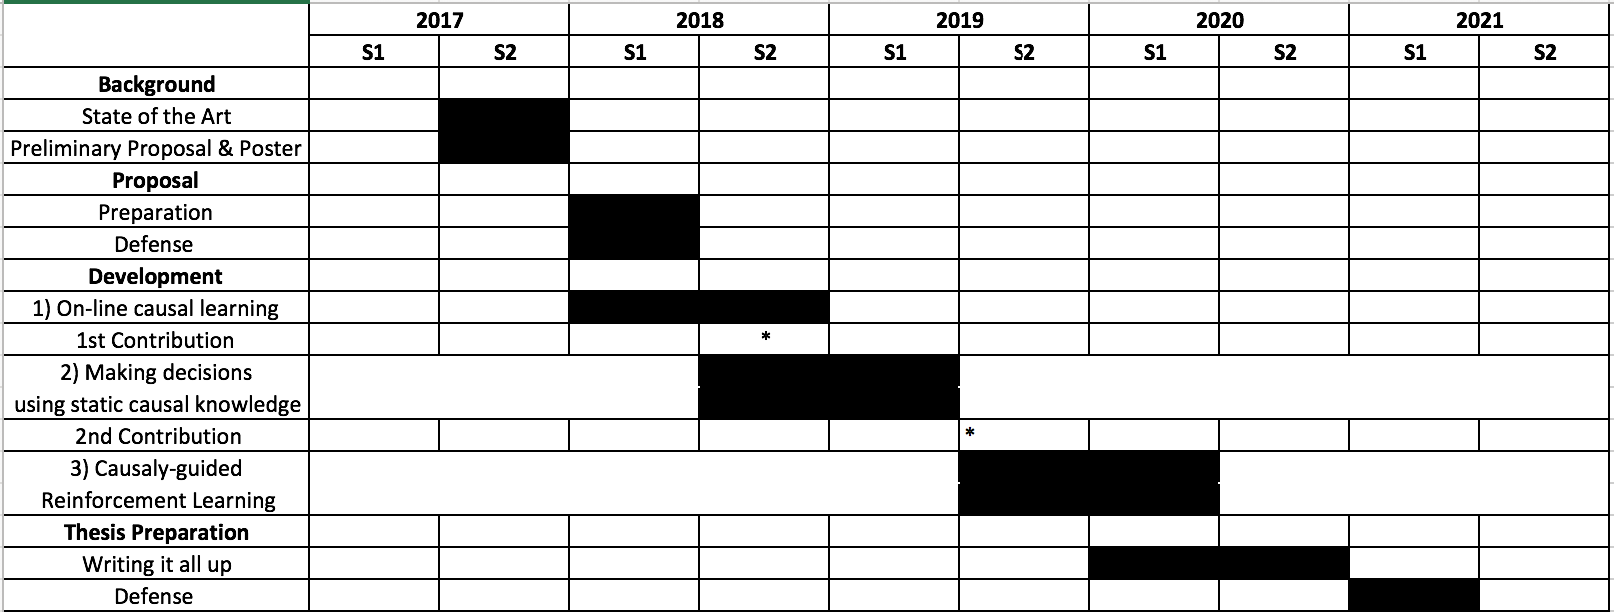
\includegraphics[scale=0.5]{Gantt.eps}
\caption{Gantt Diagram for the proposed research}
\label{causal_model}
\end{center}
\vskip -0.2in
\end{figure}


\newpage
\section{Preliminary Results}
To show the factibility of this proposal, we considered a test scenario and two cases in ascending difficulty.
\subsection{Test scenario}
Consider a sick patient who arrives at a hospital and he either has disease $A$ or disease $B$. The doctor can either give him some pill or send him into surgery.  Both treatments entail risks and whether the treatment cures the patient or not depends on which disease it had originally. The doctor could be facing a mutation from a known disease, so she has some knowledge about what could happen if a treatment is given to the patient. Using her previous knowledge as a true model, she can choose a treatment and observe the outcome from which she will learn about this disease, so she could make a better decision the next time a similar patient arrives.

The causal model that governs this situation is shown in Figure \ref{causal_model}. The parameters for this model were fixed intuitively in such a way that each treatment is effective for only one disease, but the most effective treatment is riskier.

The variables in the model are: 
\begin{itemize}
\item \textbf{Disease:} Either $A$ or $B$.
\item \textbf{Treatment:} Either pill or surgery.
\item \textbf{Reaction:} Either dying or surviving.
\item \textbf{Lives:} Either living or dying.
\end{itemize}

The variables are causally related as shown in Figure \ref{causal_model}.

\begin{figure}[ht]
\vskip 0.2in
\begin{center}
\centerline{\includegraphics[width=0.7\textwidth]{/Users/MauricioGS1/INAOE/Propuesta/Formato/figures/causal_graph.eps}}
\caption{Causal graphical model for the test scenario: the target variable \textit{Lives} is causally influenced by the disease the patient has, the treatment assigned and the survival to the secondary effects of treatment.}
\label{causal_model}
\end{center}
\vskip -0.2in
\end{figure}

The variable \textit{Lives} is the \textit{target variable} and, in this example, the only variable that can be intervened upon is the variable \textit{Treatment}. The decision maker prefers an outcome in which the patient lives.

In this scenario, Nature's move will consist in randomly assigning a disease to the patient. Then, the medic will asign a treatment using his current beliefs about the disease and the possible outcomes. The decision nodes for this play of the medic form an \textit{information set} because the medic doesn't know how she arrived there since she doesn't know what disease did Nature assign. Finally, Nature will sample the consequence of the treatment from the causal model and the medic will observe the outcome.

For this test scenario whose causal graphical model is shown in Figure \ref{causal_model}, we see  by applying the Pearl's do-calculus that the interventional distribution $P_{do(Tr)}(Y)$ is given by
\[ P(Y | do(Tr))=P(Y | D, Tr, R)P(R | Tr) P(D). \]
\\
In fact, from the structure of the model, which is shown in Figure \ref{causal_model}, we see that the involved probabilities in any calculations are:
\[ P(\textrm{disease}), P(\textrm{treatment}), P(\textrm{reaction} | \textrm{treatment}), \]
and
\[P(\textrm{lives} | \textrm{disease, treatment, reaction}). \]
\\
We can also see that the joint distribution for all of the variables can be expressed as
\[ P(Y | D, Tr, R)P(R | Tr) P(D)P(Tr). \]
This expression will be useful when specifying beliefs about the model as probability distributions.

\subsection{Case 1: The causal model is completely known}
If the causal model is completely known to the decision maker, then in one step she can obtain the probability for her desired value of the target variable, which in this case is the value corresponding to the outcome in which the patient lives at the end. Using this probability, she can choose which treatment to assign. Since this action maximizes the probability of the occurence desired value, it maximizes the expected utility, and it is also a \textit{best response} to the player Nature.

\subsection{Case 2: Only the structure is known}
Since the decision maker knows the graph structure, he can explicitly find a non interventional expression for the interventional distribution and update his beliefs about these unknown quantities. If the decision maker were not allowed to know, at the end of each round, the play of the Nature then this will have to be estimated as a hidden variable using, for example, the EM algorithm \cite{dempster1977maximum}, but meanwhile we are assuming that this information is available at the end of each round.

Given the structure of the model; i.e., the variables in it and the directed edges, the joint distribution of those variables can be expressed as a product of the form $P(X_j | Pa(X_j))$ where $Pa(X_j)$ are the parents of $X_j$ in the underlying DAG in $\mathcal{G}$. Since these distributions fully characterize the model, the decision maker will have beliefs over each one of these parameters. Notice that each of these parameters is itself a distribution of length equal to the number of possible values of the variable which is being conditioned, call the maximum number of possible values $k$ . 

A distribution suitable to modelling discrete probability vectors is the $k$-dimensional Dirichlet distribution, whose support is the set of probability vectors of length $k$ \cite{hjort2010bayesian}. The $k$ dimensional Dirichlet distribution has a density $f$ with respect to the Lebesgue measure given by

\[ f(x_1,...,x_k | \alpha_i,...,\alpha_k)=\frac{1}{B(\alpha)}  \prod_{i=1}^k x_i^{\alpha_i-1}\]

where $(x_1,...,x_k)$ are such that $\sum_{i=1}^k x_i =1$ and $\alpha=(\alpha_1,...,\alpha_k)$. The Dirichlet distribution is useful since it is conjugate for itself \cite{bernardo2000bayesian}.

The decision maker will have beliefs about the CPT's in the form of parameters of several Dirichlet distributions. Using the agent's current beliefs, a causal graphical model can be specified. Using this fully specified (structure + parameters) as a true model, the decision maker will make his choice as in Case 1. When the decision maker observes the value of the target variable, he will update the parameters that specify his beliefs.

Previously we argued that the agent's beliefs were going to be \textit{distributions} over a suitable space, but what is going to be updated are the parameters of such distributions. Namely, the $\alpha$ corresponding to the Dirichlet random variable assigned to each CPT.

For the belief updating, given a new data point,  two cases must be considered:
\begin{itemize}
\item The variable to update has no parents.
\item The variable to update has parents.
\end{itemize}

In the first case, if a prior Dirichlet($\alpha$) is used, then the posterior is given by
\[ \textrm{Dirichlet}(\alpha + c) \]
where $c$ is a vector of the number of occurrences of that observed data point. 

For the second case, we must consider both the occurrences of that data point as well as the parents for each of the variables. Following \cite{barber2012bayesian} we denote as $\theta_i(X,j)$ the number of times the event $\{X=i | Pa(X)=j\}$ is observed. In this case, if the prior of $X_i$ conditioned on its parents having the value $j$ is given by a a Dirichlet($\alpha$), then the posterior for the variable $X_i$ given an observed data point is given by 
\[ \prod_j \textrm{Dirichlet}(\alpha + \theta_i(\cdot,j)). \]

\subsubsection{Implementation}
We begin with a random assignment of the $\alpha$ parameter for each of the distributions considered. We use Dirichlet distribution for each of the conditional probability tables that appear in the factorization of the joint probability for the graph of $\mathcal{G}$. Since each of the variables in the model is binary, then the product of these Dirichlets is Dirichlet.

With this parameters, the decision maker forms a causal model and chooses the action that maximizes the probability of the desired value for target variable as in Case 1.  With this action chosen, we simulate an outcome from the causal graphical model using the chosen action as an intervention. This evidence is used to update the parameters, which then will be used to generate a new causal model, and so on.

We show the results of two experiments. We compare the performance obtained by the causal agent, a \textit{random agent} who selects his actions at random, and an agent performing Q-learning (\cite{watkins1992q}). Q-learning was chosen since it learns an \textit{optimal policy} in the sense of the Bellman Equation (\cite{sutton1998reinforcement}) and it is shown in \cite{webb2007game} that such optimal policies also maximize expected utility. 

The average performance over $20, 50, 100$ and $200$ rounds is shown in Figure 2 - 5.

\begin{center}
\begin{minipage}{0.48\linewidth}
\includegraphics[width=\linewidth]{/Users/MauricioGS1/INAOE/Propuesta/Formato/figures/20_rounds_format.eps}
\captionof{figure}{Average reward in 20 rounds}
\end{minipage}%
\hfill
\begin{minipage}{0.49\linewidth}
\includegraphics[width=\linewidth]{/Users/MauricioGS1/INAOE/Propuesta/Formato/figures/50_rounds_format.eps}
\captionof{figure}{Average reward in 50 rounds}
\end{minipage}
\end{center}
\begin{center}
\begin{minipage}{0.49\linewidth}
\includegraphics[width=\linewidth]{/Users/MauricioGS1/INAOE/Propuesta/Formato/figures/100_rounds_format.eps}
\captionof{figure}{Average reward in 100 rounds}
\end{minipage}
\hfill
\begin{minipage}{0.49\linewidth}
\includegraphics[width=\linewidth]{/Users/MauricioGS1/INAOE/Propuesta/Formato/figures/200_rounds_format.eps}
\captionof{figure}{Average reward in 200 rounds}
\end{minipage}
\end{center}

We observe that when the number of rounds is small, as in Figure 2, Q-learning outperforms our method, which achieves similar performance than the random-acting agent. On the other hand, in 50 rounds (Figure 3), our Causal Agent and the Q-Agent have left behind the Random Agent, which is even more noticeable by 200 rounds. This means that our agent (Causal Agent) is both learning a good action while learning a Causal Model of the environment that he is facing.

\subsection{Case 3 and future work: The model is not known}
The causal model were fully unknown, the decision maker will have to deal with the problem using only any previous knowledge and her own intuitions. Again, any previous knowledge and considerations will be expressed as \textit{beliefs} about the uncertainties in the environment, which will take the form of a probability distributions over a suitable space. 

As in the previous case, we consider a repeated game where the base game consists of Nature assigning a random state of the environment and responding to the agents choices with the effects that were caused by her decisions. In this game, as well as in the previous one, the decision maker will attempt to learn by updating, and using, beliefs in a suitable way. 

The most notable difference with the previous case is that the \textit{structure} of the model is also to be learned in such a way that both the structure and parameters converge to the true model in the limit. In the previous case the decision maker knew the form of the Conditional Probability Tables (CPT) involved in any calculation. In this case, she doesn't know the structure of the DAG so which CPT's are involved is unknown.

If the decision maker knew which variables appear in the true model that governs the environment, even though she didn't know how they are connected, she could use a \textit{Dirichlet Process} to generate Dirichlet distributions and generate causal graphical models the same way as in Case 2 and updating the parameters of the process using the observed information. The Dirichlet Process\footnote{with parameters $M,G_0$}, which was introduced by \cite{ferguson1973bayesian}, is random measure defined over a space $S$ such that for each partition $B_1,...,B_k$ the vector $(G(B_1),...,G(B_k))$ follows a Dirichlet distribution \cite{hjort2010bayesian}, \cite{muller2016bayesian}, \cite{ghosal2017fundamentals}. 

Belief updating using causal information when the decision maker current knowledge is specified as a Bayesian Nonparametric Prior (BNP)  is yet to be studied and left as future work, since the construction and use of this kind of priors is a hard problem, this is because a BNP is basically a probability distribution over infinite-dimensional spaces, such as the space of continuous functions or the space of unbounded graphs (\cite{hjort2010bayesian}, \cite{phadia2015prior}, \cite{ghosal2017fundamentals}).
\newpage
\section{Conclusions}
We have proposed that an autonomous, rational agent who faces an uncertain environment which is governed by an unknown causal mechanism can make use of the causal relations that hold in such environment in order to find an action that will take him into the way of a desired result, in terms of his (rational) preferences. Also, causal information can be acquired while interacting with the environment and this newly acquired information will enrich the decision making procedure. 

We have taken inspiration in how human beings use causal information when interacting with the world, which has a complex causal structure, in order to pursue objectives. Following this intuitions we proposed a \textit{guiding principle} to exploit causal information that must be followed by a rational agent in order to be coherent with the definition of rationality. From the guiding principle we stated a systematic approach into causal decision making and considered three cases to be solved in order. In two of the three cases we showed that a performance similar to classical decision-making algorithms can be achieved while also learning a causal model from the environment. We are considering. If this research is allowed to continue, we will delve into general settings that resemble realistic situations in which the causal model that controls an environment is barely known.
\newpage
%------------- References --------------------
\singlespacing
%doi=false,isbn=false,url=false
\bibliographystyle{apalike}
\bibliography{/Users/MauricioGS1/INAOE/Propuesta/Bibliografia.bib}

%------------- Apendice --------------------


\end{document}